% ****************************************************************************************** % Dissertation template and document class
% Author  : 
% ****************************************************************************************** %
%%% For print copies
%% set 'singlespace' option to set entire thesis to single space, and define "\printmode" to remove all hyperlinks for printed copies of the thesis. Delete all output files before changing this mode -- it will turn hyperref package on and off
%\newcommand{\printmode}{}

%%% For the electronic copy, use doublespacing, define "\proquestmode" to use outlined links, instead of colored links. 
\documentclass[report,a4paper,12pt]{pieasthesis}
\newcommand{\proquestmode}{} %\printmode or \proquestmode
\title{AI Frameworks for Visual Traffic Surveillance, from Vehicle Classification to Event Detection}

\submitted{Januray 3, 2020}  % degree conferral date (January, April, June, September, or November)
\copyrightyear{2011}  % year in which the copyright is secured by publication of the dissertation.
\author{Assad Sultan \\ \& \\ Muneeb ur Rehman}
\adviser{Dr. Zulfiqar Hassan}  %replace with the full name of your adviser
%\departmentprefix{Program in}  % defaults to "Department of", but programs can change this.
\department{Electrical Engineering}
\degreeprefix{BS}
\degree{Electrical Engineering}
%%%%%%%%%%%%%%%%%%%%%%%%%%%%%%%%%%%%%%%%%%%%%%%%%%%%%%%%%%%%%\
    \renewcommand{\topfraction}{0.85}	% max fraction of floats at top
    \renewcommand{\bottomfraction}{0.6}	% max fraction of floats at bottom
    \setcounter{topnumber}{2}
    \setcounter{bottomnumber}{2}
    \setcounter{totalnumber}{4}     % 2 may work better
    \setcounter{dbltopnumber}{2}    % for 2-column pages
    \renewcommand{\dbltopfraction}{0.66}	% fit big float above 2-col. text
    \renewcommand{\textfraction}{0.15}	% allow minimal text w. figs
    %   Parameters for FLOAT pages (not text pages):
    \renewcommand{\floatpagefraction}{0.66}	% require fuller float pages
	% N.B.: floatpagefraction MUST be less than topfraction !!
    \renewcommand{\dblfloatpagefraction}{0.66}	% require fuller float pages
    

\usepackage{graphicx,verbatim,amsmath,multirow,longtable,booktabs,epsfig,epstopdf,multicol}
\setlength{\LTcapwidth}{\textwidth}
\usepackage[top=1in, bottom=1in, left=1.5in, right=1in]{geometry}
\usepackage[utf8]{inputenc}
\usepackage{float} 
\usepackage{fullpage}
\usepackage{pbox}

%%%%%%%%%%%%%%%%%%%%%%%%%%%%%%%%%%%%%%%%%%%%%%%%%%%%%%%%%%
%%% Printed vs. online formatting
\ifdefined\printmode
% Printed copy\usepackage{array}
\usepackage{makecell}

\renewcommand\theadfont{\normalsize\bfseries}
% url package understands urls (with proper line-breaks) without hyperlinking them
\usepackage{url}
\else
\ifdefined\proquestmode
\usepackage[hidelinks]{hyperref}
\hypersetup{bookmarksnumbered}
\makeatletter
\hypersetup{pdftitle=\@title,pdfauthor=\@author}
\makeatother

\else
\usepackage{hyperref}
\hypersetup{colorlinks,bookmarksnumbered}

% copy the already-set title and author to use in the pdf properties
\makeatletter
\hypersetup{pdftitle=\@title,pdfauthor=\@author}
\makeatother

% make the page number rather than the text be the link for ToC entries
%\hypersetup{linktocpage}
\fi % proquest or online formatting
\fi % printed or online formatting
\usepackage{sectsty}
\usepackage{lipsum}
\subsectionfont{\fontfamily{phv}\itshape\normalsize}
\subsubsectionfont{\normalsize}
\sectionfont{\large}
%\subsectionfont{\sffamily\itshape}
\setcounter{secnumdepth}{4} 
\setcounter{tocdepth}{4}
%%%%%%%%%%%%%%%%%%%%%%%%%%%%%%%%%%%%%%%%%%%%%%%%%%%%%%%%%%%%%\
%%%% Define commands

\newenvironment{indenttext}{
    \begin{list}{}{ \itemsep 0in \itemindent 0in
    \labelsep 0in \labelwidth 0in
    \listparindent 0in
    \topsep 0in \partopsep 0in \parskip 0in \parsep 0in
    \leftmargin 1em \rightmargin 0in
    \raggedright
    }
    \item
  }
  {\end{list}}

% another environment that's an indented list, with no spaces between items -- if we want multiple items/lines. Useful in tables. Use \item inside the environment.
% 	\raggedright makes them left aligned instead of justified
\newenvironment{indentlist}{
    \begin{list}{}{ \itemsep 0in \itemindent 0in
    \labelsep 0in \labelwidth 0in
    \listparindent 0in
    \topsep 0in \partopsep 0in \parskip 0in \parsep 0in
    \leftmargin 1em \rightmargin 0in
    \raggedright
    }

  }
  {\end{list}}
%%%%%%%%%%%%%%%%%%%%%%%%%%%%%%%%%%%%%%%%%%%%%%%%%%%%%%%%%%%%%\
%%%% Front-matter
% For early drafts, you may want to disable some of the frontmatter. Simply change this to "\ifodd 1" to do so.
\ifodd 0
% you can just skip the \acknowledgements and \dedication commands to leave out these sections.
\else
\dedication{Dedicated to our Parents for their love and affection}
% \acknowledgements{
% \chapter*{Acknowledgements}
\addcontentsline{toc}{chapter}{Acknowledgements}

I would like to thank the Math department for providing the original documentclass file that this class is based upon. I would like to thank my parents, without whom my life would not be possible. I would also like to thank my advisor, my dissertation committee, and my research collaborators because every graduate student needs to do so. And finally, I thank the members of my research group, to whom I leave this template to save you some of the trouble I had to go through getting my dissertation to compile in \LaTeX{}.  

Don't forget to ask your advisor if your work was sponsored by a grant that needs to be acknowledged in this section.  
% }
\abstract{

\chapter*{Abstract}
\addcontentsline{toc}{chapter}{Abstract}
\vspace{-3mm}
The key objective of this project is the detection \& classification of vehicles for traffic surveillance purposes.
Increasing accidents on roads have made the need of efficient methods to meet the detection \& classification
purposes significant. Several state of the art alogrithms exist which detect and classify the objects considering
some features but to acheive high precision in short time, we need robust algorithms. In the past few years, CNNs have
acheived a rapid success in accuracy and speed. In this project, a CNN based detector is used called as YOLO. The algorithm is
customized according to the requirements. The still images are used for training made available using web scrapping to make a large dataset
to get good results during training. The dataset consists of vehicles of 8 different classes. After the classification 
mechanism, detection algorithms are used for the detection of objects in a still image 
and moving frames. 
\vspace{15mm}\ \\
\textit{Keywords: Deep Learning, Detection, Vehicles, Convolutional Neural Networks, Deep Neural Networks, YOLO}

}
%%%%%%%%%%%%%%%%%%%%%%%%%%%%%%%%%%%%%%%%%%%%%%%%%%%%%%%%%%%%%\
%%%% Hide some chapters

%%% If you want to produce a pdf that includes only certain chapters, specify them with includeonly, in addition to including all chapters below.
%\includeonly{ch-intro/chapter-intro}
%%% You can also specify multiple chapters.
%\includeonly{ch-intro/chapter-intro,ch-usage/chapter-usage}
%\includeonly{chap1,chap2,chap3}


%%%%%%%%%%%%%%%%%%%%%%%%%%%%%%%%%%%%%%%%%%%%%%%%%%%%%%%%%%%%%
%%%% Notes:

% Footnotes should be placed after punctuation.\footnote{place here.}
% Generally, place citations before the period~\cite{anotherauthor}.
% The proper usage for i.e., and e.g., include commas ``(e.g., option A, option B)''
%%%%%%%%%%%%%%%%%%%%%%%%%%%%%%%%%%%%%%%%%%%%%%%%%%%%%%%%%%%%%
%%%% Import chapters
\usepackage{fancyhdr}
\usepackage{graphicx}
\usepackage{caption}
\usepackage{subfig}
\usepackage{xcolor}
\usepackage{minted}
\setminted{fontsize=\footnotesize}

\fancypagestyle{plain}{
\fancyhf{} % clear all header and footer fields 
\fancyhead[R]{\thepage} %RO=right odd, RE=right even

\renewcommand{\headrulewidth}{0pt} 
\renewcommand{\footrulewidth}{0pt}} 
\usepackage[titletoc]{appendix}
\definecolor{bg}{rgb}{0.95,0.95,0.95}

\begin{document}
\makefrontmatter

\chapter{Introduction}
\label{1}
\section{Motivation}

With the development of science and technology, there may arise crucial 
problems. Rising traffic in the country gives birth to rising accidents. To 
avoid/minimize the accidents, proper surveillance is required. Detection 
and tracking of vehicles have become a key component in traffic 
surveillance and automatic driving. Traditional algorithms like Gaussian 
Mixed Model (GMM) has achieved encouraging success in this field \cite{chap_1_article:1}. But due 
to variation in illumination, occlusion, background clutter etc. detection 
of vehicles is still a challenge. 
Deep Neural Networks (DNNs) have gained a lot of attention in 
past few years. Due to the betterment of deep learning, object 
detection has achieved major advancements in recent years. The work 
in this project is based on DNNs to detect and classify vehicles from 
a dataset collected from images and videos.

\section{Background}

Classical methods of vehicle detection were based on some 
sort of features like symmetry, edges, texture, underbody shadows 
and corners \cite{chap_1_article:2}. These methods were easy to describe and perform 
in specific kind of applications. These methods fail in many situations 
like due to less illumination of highway. With the advent of 
deep learning, a subset of machine learning, the detection and 
classification mechanism have dramatically improved. Machine learning 
and deep learning are sub-branches of computer intelligence which help 
in the process of vehicle classification to event detection. 
Using deep learing techniques, we are going to focus on a specific kind 
of detection (deep learning has grown its branches in almost every 
kind of image recongnition, text recognition, face detection etc), vehicle 
detection. Using deep learning based Convolutional Neural Networks (CNNs) 
which is a wide field for object detection, classification, sementic 
segmenation etc. These networks take input images, learn features, adjust 
weights and then detect the targets from test data. In deep learning, 
algorithms automatically learn features unlike machine 
learning algorithms, we have to pass features to train the 
model. Our work is based on Deep Neural Networks (DNNs).

\section{Goals \& Objectives}

The goal of this project is to make a deep learning based model (using Python) for vehicle detection and classification. Main objectives are summarized as:
\begin{itemize}
\item Collection of datasets (images dataset of car, truck classes etc. and videos).
\item Design of Convolutional Neural Network
\item Configuration of training options (AlexNet, VGGNet, ResNet etc.)
\item Training of detector (RCNN, Fast- RCNN, Faster-RCNN, YOLO etc.)
\item Evaluation of the trained detector
\end{itemize}

\section{Challenges}

Human can understand and interpret images in a 
second or less. For machines, it is not easy to achieve 
accurate results unless models are trained properly. Firstly, proper 
training is a challenging task for a customized data. Detection 
algorithms are also hard to implement as we must have recommended 
GPU requirements and best choice of algorithm for good results. Videos 
which are moving frames, it is difficult to draw accurate bounding boxes 
in a video having say 30 frames per second 
means 30 images are splashed in a second. 	


\section{Organization of Thesis}

\textbf{Chapter \ref{Chapter 2}}: Chapter 2 is about literature review. It is about
the whole reading and understanding of Image classification \& detection.

\noindent\textbf{Chapter \ref{Chapter 3}}: This chapter is about Convolutional Neural Networks. All CNN architectures with their details
are discussed.



% \begin{figure}[H]
% 	\centering
% 	%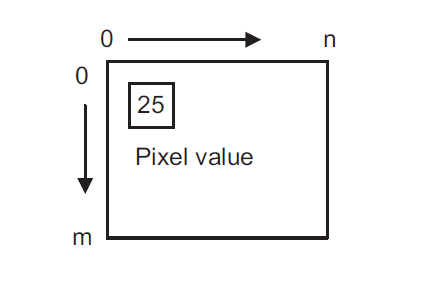
\includegraphics[scale = 0.5]{CHAPTERS/Chapter-2/Images/2.2.png}
% 	\caption{Grayscale Image format}
% 	\label{fig:1.1}
% \end{figure}
\chapter{Literature Review}
\label{Chapter 2}

\section{History of Object Recognition \& Detection}

The field of computer vision deals with how the computers can be made to understand digital images or videos. 
The history of Computer Vision can be traced back to 1960s. Before that people had tried for alphabet recognition 
but those attempts had not led very far. L.G. Roberts, in his Ph.D thesis mentioned about the perception 
of solid objects. Using the properties of three dimensional transformations and the laws of nature, a procedure 
was developed which had been able to identify objects as well as determine their orientation and position in space \cite{chap_2_article:1}. 

In 1970s, David Marr wrote a book on visual recognition. In his book he mentioned that in order to take an 
image and to arrive at a final holistic full 3D representation of the visual world, we must go through 
several processes. The first process he calls is “Primal sketch” where edges, bars, ends and virtual lines 
are determined. Next is “two and half-D sketch” leading to “3-D sketch”  \cite{chap_2_article:2}. Another very important seminal 
group of work happened in 1970s when people began to ask the question, “how can we move beyond simple block 
world and start recognizing real objects?” Two group of scientists proposed similar ideas, one 
is called “generalized structure” and other is called “pictorial structure”. The basic idea was that 
every object is composed of simple geometric primitives \cite{chap_2_article:3}. 

In 80s, David Lowe tried to recognize razors by constructing lines and edges and mostly straight lines 
and their combination. At those times, it was very hard to solve an image recognition problem due to 
limited resources. From 1999 to 2000, statistical machine learning techniques started to gain momentum. Such 
techniques are support vector machines, boosting, graphical models etc. In 2006, FujiFilm rolled out first 
digital camera with face detection feature.

One of the very influential way of thinking in the late 90s till the first 10 years of 21st century was feature 
based recognition. An important work was done by David Lowe based on a feature called as SIFT feature. The idea 
was that to match one stop sign shown in Figure \ref{fig:2.1} with another stop sign is very difficult, because there might 
be all kinds of changes due to camera angles, occlusion, viewpoint, lighting and just the intrinsic variation of 
the object itself. Despite it is inspired to observe that there are some parts of the object that tend to remain 
unchanged. So, the task of object recognition began with identifying those features on the object and match these 
features to a similar object \cite{chap_2_article:4}.

\begin{figure}[t]
	\centering
	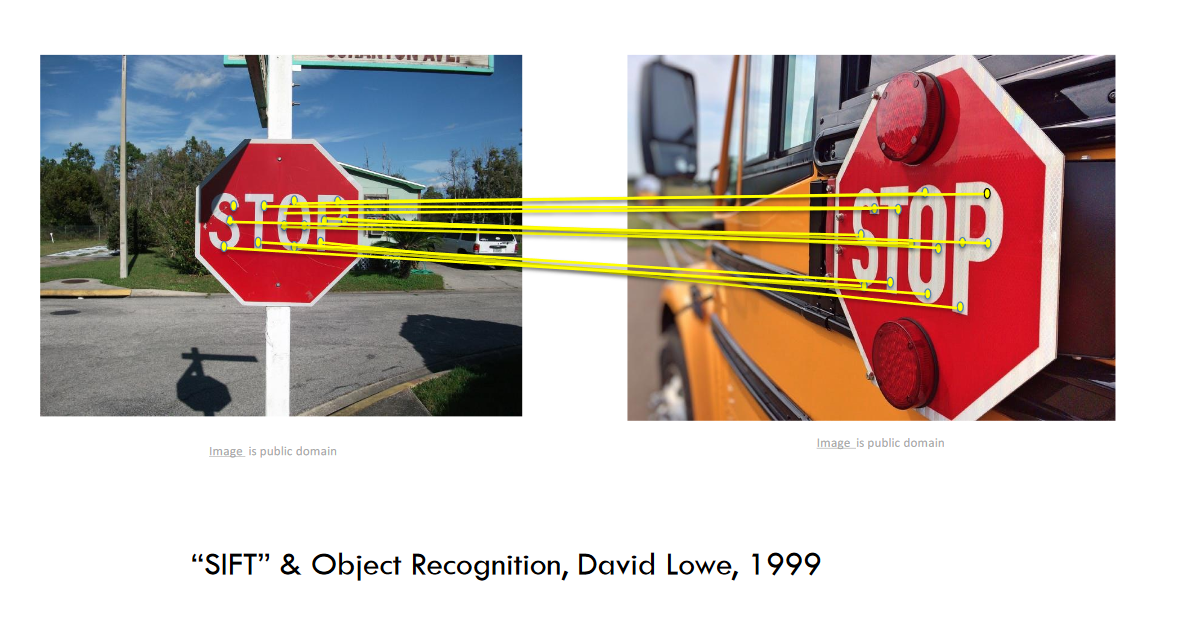
\includegraphics[width=0.80\textwidth]{CHAPTERS/Chapter-2/Images/2.1.png}
	\caption{SIFT \& Object Recognition}
	\label{fig:2.1}
\end{figure}
In 2009, the ILSVRC was 
rolled out. This data set contains 1.4 million images of different classes. In 2012, the 
error rate was dropped to almost 16 \% \cite{chap_2_article:5}. The winning algorithm was based on 
CNNs. This work was published in 2012 introducing AlexNet, which brought a tremendous change in the field of image recognition. This thesis is based on image 
classification and detection using CNNs. 

\section{Basics of an Image}
To start with, we must understand all about an image, the information of 
an image that is important to a machine. A digital image is picture 
information in digital form. It consists of pixels. The number of pixels 
in the presentation of a digital image is its spatial resolution, which 
relates to the image quality. The higher the spatial resolution, the better 
quality the image has. The resolution can be high, for instance, as high as 
1,600 $\times$ 1,200 (1,920,000 pixels = 1.92 megapixels), or as 
low as 320 $\times$ 200 (64,000 pixels = 64 kilo pixels). In notation, the number 
to the left of the multiplication symbol represents the width, and that to 
the right of the symbol represents the height. Image quality also depends on 
the numbers of bits used in encoding each pixel level \cite{chap_2_article:6,chap_2_article:7}. 

\subsection{8-Bit Gray Level Images}
If a pixel is encoded on a gray scale from 0 to 255, where 
0 corresponds to black and 255 corresponds to white. The intermediate 
numbers represent the shades of gray. For example, for a 640 $\times$ 480 bit 
image, 307.2 kilobytes are required for storage. Figure \ref{fig:2.2} shows a 
grayscale image format. The pixel value indicated 
in the box has an 8-bit value of 25. 

\begin{figure}[H]
	\centering
	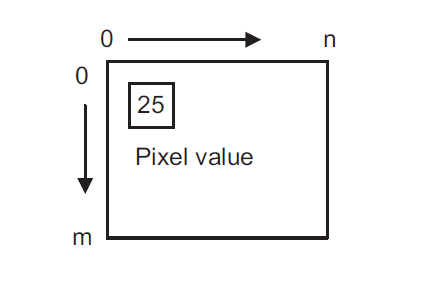
\includegraphics[scale = 0.5]{CHAPTERS/Chapter-2/Images/2.2.png}
	\caption{Grayscale Image format}
	\label{fig:2.2}
\end{figure}

\subsection{2.2	24-bit Color Images}
In a 24-bit color representation, each pixel of an image is 
encoded with Red (R), Green (G) and Blue (B) values. With each component 
encoded in 8 bits, we have a total of 24 bits for a full color RGB image. Having 
such an image, we have 2\textsuperscript{24} = 16:777216 $\times$ 10\textsuperscript{6} 
different colors. A 640 $\times$ 480 24-bit color 
image requires 921.6 kilobytes for storage. Figure 2.3 shows the format for the 24-bit 
color image where the indicated pixel has 8-bit RGB components.

\begin{figure}[H]
	\centering
	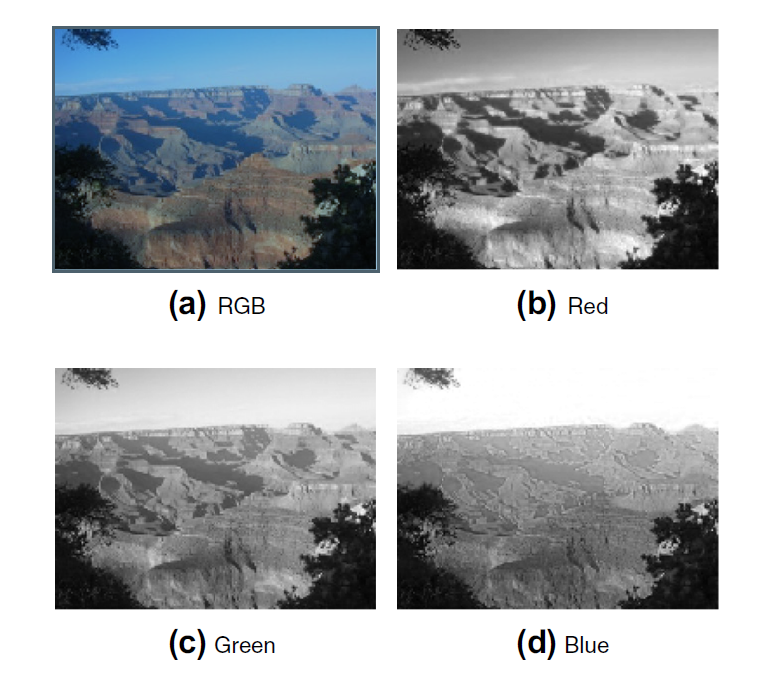
\includegraphics[width=0.80\textwidth]{CHAPTERS/Chapter-2/Images/2.3.png}
	\caption{The 24-bit color image and its RGB components}
	\label{fig:2.3}
\end{figure}

\subsection{8-Bit Color Images}
The 8-bit color image is also a popular image format. The pixel 
values are indexed from 0 to 255. Each index represents an entry of the 
color map. These images are called color indexed images. As an example, figure 2.4 shows 
a color indexed image that has a pixel value of 5, which is the index for the entry of 
the color table. At location 5 in the color table, there are three color components with 
RGB values of 66, 132 and 134 respectively. Each color component is encoded in 8 bits. There are 
only 256 different colors in the image. A 640 $\times$ 480 8-bit color image requires 307.2 kilobytes 
for data storage and 3 $\times$ 256 = 768 bytes for color map storage.

\begin{figure}[H]
	\centering
	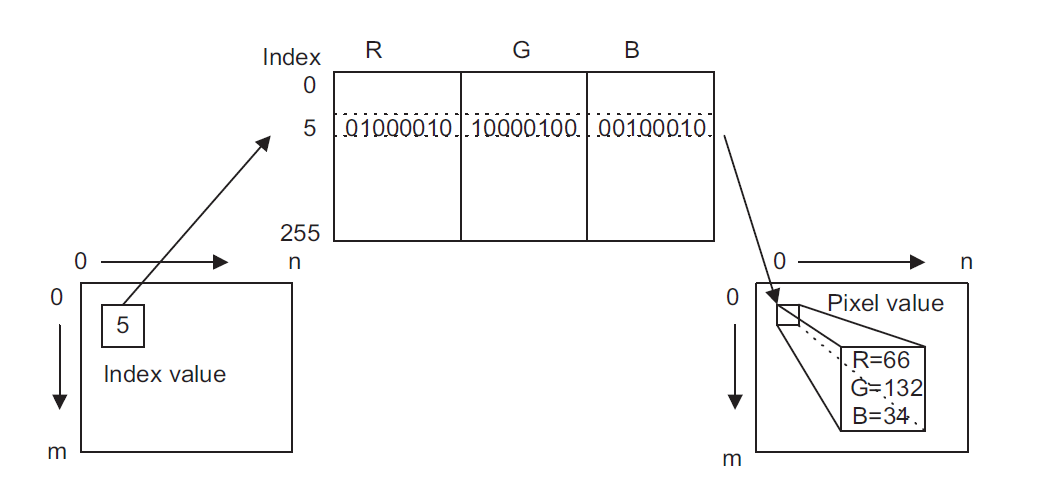
\includegraphics[width=0.80\textwidth]{CHAPTERS/Chapter-2/Images/2.4.png}
	\caption{The 8-bit color indexed image}
	\label{fig:2.4}
\end{figure}

\subsection{Intensity Images}
In section 2.1, we mentioned that a grayscale image uses a 
pixel value in the range 0-255. A 0 value represents black while 255 
represents white. In some processing environments, floating point representations 
are used. The grayscale image has an intensity value normalized from 0 to 1, where 0 is 
for black and 1 is for white. Figure 2.5 shows the format of the grayscale intensity 
image, where the indicated pixel shows the intensity value of 0.5988.

\begin{figure}[H]
	\centering
	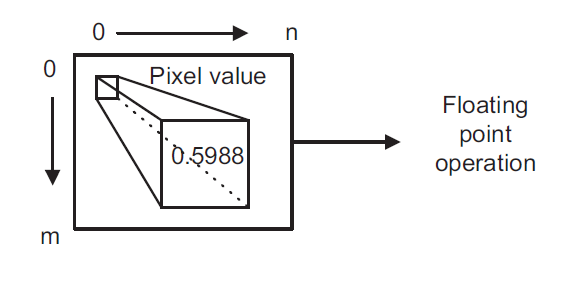
\includegraphics[scale = 0.75]{CHAPTERS/Chapter-2/Images/2.5.png}
	\caption{The grayscale intensity image format}
	\label{fig:2.5}
\end{figure}

\subsection{Red, Green, and Blue Components and Grayscale Conversion}

For processing applications, we often need to convert RGB image to grayscale. There are two popular methods, one is average method where a grayscale value is obtained by just averaging the red, green and blue pixel values. The other is luminosity method, where we use approximately 30 \% of Red, 59 \% of Green and
11\% of Blue to form a grayscale image.
\begin{equation}
	\mbox{New grayscale image} = 0.3R + 0.587G + 0.114B
\end{equation}
\section{Image Classification}
Humans can understand and depicts the information contained in an image. On the other 
hand, machines cannot identify the image and retrieve information from it on its own. To 
achieve that purpose, we make the machines learn from examples and when it has learned 
enough, it may extract information from an image from an outside world and recognize it.

There exist many algorithms for image classification. One of them is BoW 
model, which is commonly used for document classification and natural language 
processing. In addition to document classification, the BoW model can also be used for 
image classification. We extract a set of features from an image and count 
their occurrence. We have different algorithms for feature extraction. For example, in 
BoW model, SURF algorithm was used \cite{chap_2_article:8}. Other interesting image 
classification methods include texture analysis. However, a gain in performance has been 
brought by using neural networks. With the introduction of AlexNet architecture in 
2012, the error rate was dropped tremendously. Due to robustness of these 
algorithms, the CNNs are widely used for 
image classification and recognition nowadays. 

The problem of image classification can be stated as: \textit{“Given a set of 
images labeled with a single category, the machine has to predict a new set 
of images by assigning it a label and test the accuracy of the predictions”}. For 
example, in Figure \ref{fig:2.6} an image classification model takes a single image and assigns 
probabilities to 4 labels, {cat, dog, hat, mug}. The computer sees the image as a 
3D-array of numbers. The cat example image is 248 pixels wide and 400 pixels in height 
with three color channels, Red, Blue and Green, therefore, a total 
of 248 $\times$ 400 $\times$ 3  = 297,600 numbers. Each number is an integer with values 
in range 0-255. What our task is to extract out of these 
thousands of numbers, a single label, such as “cat”. 

\begin{figure}[H]
	\centering
	\captionsetup{justification=centering,margin=2cm}
	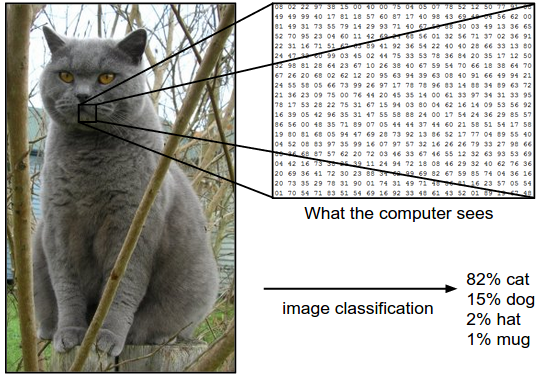
\includegraphics[width=0.80\textwidth]{CHAPTERS/Chapter-2/Images/2.6.png}
	\caption{A 3D-array of numbers from 0 to 255 of size width $\times$ height $\times$ 3. 3 represents color channels}
	\label{fig:2.6}
\end{figure}

There are a variety of challenges associated with this. There 
may exist viewpoint variation, scale variation, deformation, occlusion (a small portion 
of object is displaying), illumination conditions, background clutter and intraclass 
variations. How do we end up writing an algorithm for image classification? Researchers have 
arrived at the point that in order to solve this problem, use data-driven approach. Instead 
of writing a code to specify everyone categories of interest look like, we provide computer 
many examples of images of each class and then develop the algorithm that look at these 
examples and learn about the visual representation of each class. This approach is known 
as data-driven approach. So, the image classification pipeline can be summarized as:

\begin{itemize}
\item Input of the system is a training dataset composed 
of N images of labeled with K different classes.
\item Using this training set, we train a classifier to learn how do these classes look like.
\item After that, test this classifier on a new dataset and then compare the results with the true labels of the images.
\end{itemize}

\subsection{Convolutional Neural Networks}

CNNs are the most famous network used 
for classification problems of images. The idea behind CNNs is that a 
local understanding of an image is good enough. A practical advantage is 
that if we have fewer parameters, it will reduce the amount of data to train 
a model and improves the time of learning. A CNN has weights to look at a small 
patch of image. 

A convolution is a weighted sum of  the pixel values of an image, as 
we have a sliding window moving across the whole image. It produces another 
image of the same size. A CNN typically consists of 3 layers:

\begin{enumerate}
	\item Convolution Layer
	\item Pooling Layer
	\item Fully Connected Layer

\end{enumerate}
There are some batch normalization layers in some old CNNs 
but not used these days. (Details of CNNs are covered in chapter 3).

\subsubsection{CNN Architectures}
As mentioned before, the ImageNet project is a large visual database designed for research purposes. This 
project runs on an yearly contest named as ILSVRC, where different algorithms compete 
to classify and detect objects. Here 
we will talk about the competition top competitors \cite{chap_2_article:9}.
\begin{itemize}
	\item LeNet-5 (1998)
	\item AlexNet (2012)
	\item ZFNet (2013)
	\item GoogleNet (2014)
	\item VGGNet (2014)
	\item ResNet (2015)
\end{itemize}
\paragraph*{LeNet}

It is a pioneering 7-layer convolutional network by 
Yann LeCun et al. in 1998. It classifies digits and was applied by 
several banks to recognize handwritten numbers on cheques. The processing 
of higher resolution images we need more convolutional layers, so this 
technique is constrained by the availability of resources \cite{chap_2_article:10}.

\begin{figure}[H]
	\centering
	\captionsetup{justification=centering,margin=2cm}
	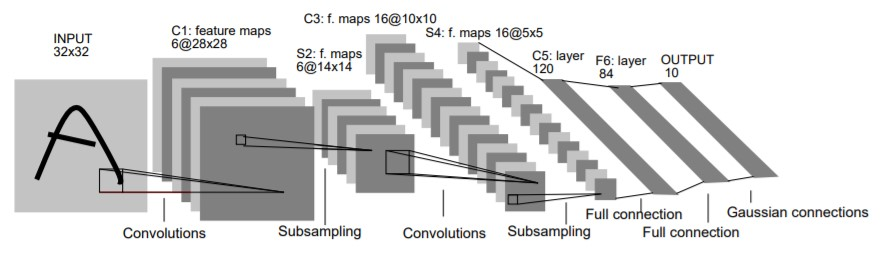
\includegraphics[scale= 0.8]{CHAPTERS/Chapter-2/Images/2.7.jpg}
	\caption{Architecture of LeNet-5, original image published in [LeCun et al., 1998]}
	\label{fig:2.7}
\end{figure}


\paragraph*{AlexNet (2012):}
In 2012, Krizhevsky et al. introduced AlexNet which 
outperformed all the prior competitors and won the challenge 
by reducing the error to 15.3 \%.  This network had a similar architecture 
like LeNet but was deeper with more filters per layer. It 
consists of 11 layers between input and output. 

 
\begin{figure}[H]
	\centering
	\captionsetup{justification=centering,margin=2cm}
	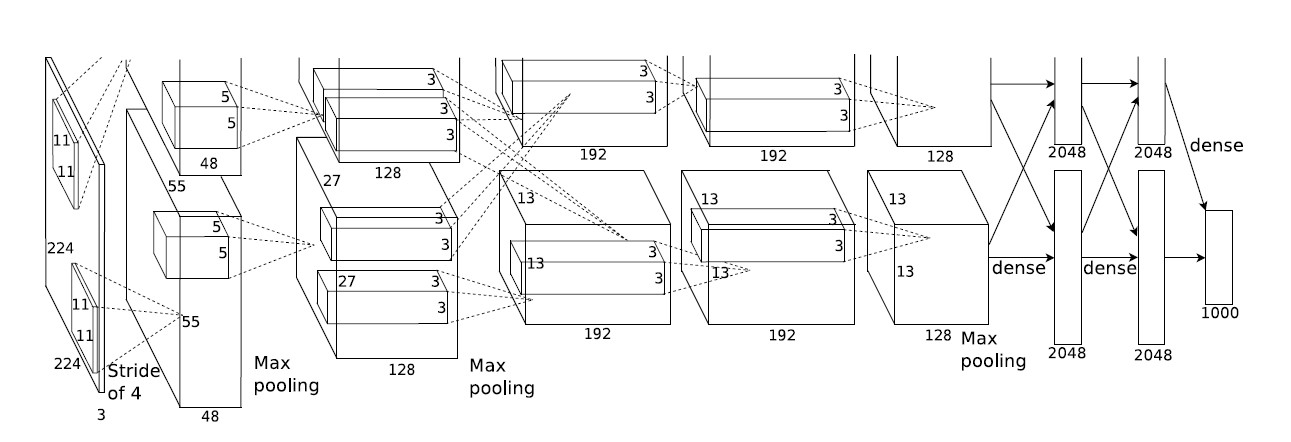
\includegraphics[scale = 0.6]{CHAPTERS/Chapter-2/Images/2.8.jpg}
	\caption{An illustration of the architecture of AlexNet CNN}
	\label{fig:2.8}
\end{figure}

\paragraph*{ZFNet (2013):}
This architecture was the winner of 2013 ILSVRC. It achieved 
an error rate of 14.8 \%. It was achieved by tweaking the 
hyperparameters of AlexNet while maintaining the same structure and 
adding deep learning elements \cite{chap_2_article:11}. The architecture 
is shown in \ref{fig:2.9}.

\begin{figure}[H]
	\centering
	\captionsetup{justification=centering,margin=2cm}
	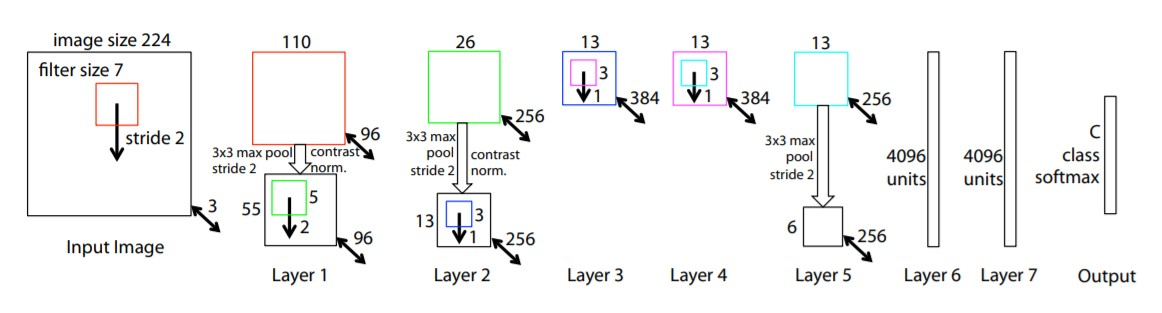
\includegraphics[scale = 0.6]{CHAPTERS/Chapter-2/Images/2.9.jpg}
	\caption{Architecture of 8 layer ZFNet Model}
	\label{fig:2.9}
\end{figure}

\paragraph*{GoogleNet (2014):}
This architecture was the winner of  ILSVRC, 2014. It achieved a top-5 
error rate of 6.67 \%. It was close to human level performance. The network 
was inspired by LeNet but implemented a new element which is dubbed an 
inception module. It used batch normalization, image distortions and RMSprop. This architecture consists of 22 layers but a 
reduced number of parameters from 60 million to 4 million \cite{chap_2_article:12}. 

\paragraph*{VGGNet (2014):}
The VGGNet was developed by Simonyan and Zisserman. It was 
runner-up in ILSVRC, 2014. It consists of 16 convolutional 
layers and popular because of its uniform architecture. A challenging thing in 
VGGNet is that it consists of 138 million parameters \cite{chap_2_article:13}.
\begin{figure}[H]
	\centering
	\captionsetup{justification=centering,margin=2cm}
	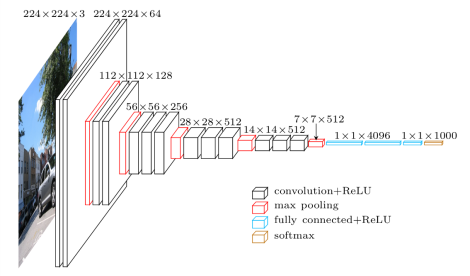
\includegraphics[scale = 0.6]{CHAPTERS/Chapter-2/Images/2.11.png}
	\caption{An illustration of the architecture of VGGNet CNN}
	\label{fig:2.10}
\end{figure}

\paragraph*{ResNet (2015):}
In 2015, Residual Neural Network (ResNet) by Kaiming He et al. was introduced. It was a novel architecture with “skip connections” and features heavy batch normalization. These connections are known as gated units. There are 152 layers but still less complex than VGGNet. It achieved a top-5 
error rate of 3.57 \% which beats human-level performance \cite{chap_2_article:14}. 

\begin{figure}[H]
	\centering
	\captionsetup{justification=centering,margin=2cm}
	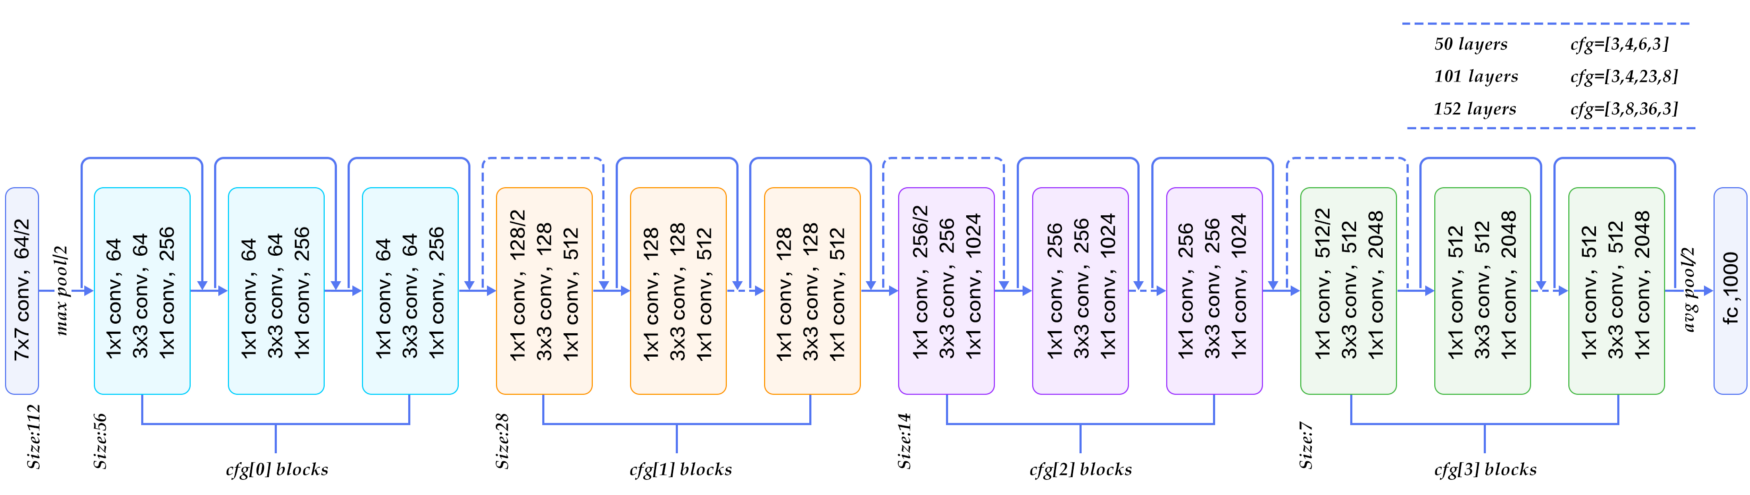
\includegraphics[width = 0.8\textwidth]{CHAPTERS/Chapter-2/Images/2.12.png}
	\caption{ResNet Architecture}
	\label{fig:2.11}
\end{figure}

AlexNet has parallel two CNN line trained on two GPUs with cross-connections, GoogleNet has 
inception modules, ResNet has residual connections.

\subsubsection*{Summary Table}
\begin{table}[H]
	\caption{Comparison of Different CNN Architectures}
	  \begin{center}
		\scalebox{.85}
		{\begin{tabular}{|l |l |l |l |l |}
		\hline
		Year & CNN & Developed by & Top-5 error rate (\%) & No. of Parameters \\ \hline
		1998  & LeNet(8) & Yann LeCun et al. &  &  60 thousand 
		\\ \hline
		2012  & AlexNet(7) & Alex Krizhevsky et al. & 60 million &
		\\ \hline
		2013   & ZFNet() &  Mathhew, Zeiler \& Rob Fergus & 9 &
		\\ \hline %
		2014 & GoogleNet(19) & Google & 6.67  & 4 million
		\\ \hline
		2014 & VGGNet(16) & Simonyan, Zisserman & 7.3 & 138 million
		\\ \hline
		2015 & ResNet(152)& Kaiming He & 3.6 & 
		\\ \hline   
		\end{tabular}}
	  \end{center}
\end{table}


\chapter{Convolutional Neural Networks (CNNs)}
\label{Chapter 3}

CNNs are types of artificial neural networks used 
for object detection and image classification etc. Neural Networks 
are brain-inspired set of algorithms that are expected to mimic the working 
of human brain. Billions of neurons in our brain process information through 
electrical signals. Dendrites receive external information or stimuli in form of 
electrical impulses which is further processed in the cell body where it integrates 
all the signals coming in and the output is carried away to the downstream neurons 
through Axons \cite{chap_3_article:1}. The neuron chooses to either reject or accept the signal 
depending on the signal strength. Likewise, an artificial neural network consists of large 
number of interconnected nodes known as neurons. The computational node and cell body of 
neuron works in kind of a similar way where we have large number of signals 
coming as inputs to neuron. Each signal has a weight W associated with it and the 
summation of these weighted inputs is passed to the activation function where 
 non-linearity is introduced in the output. Neural networks have the ability to gradually 
update the weights of the interconnections of the neuron until desirable results 
are obtained during the training phase of network.

\begin{figure}[H]
	\centering
		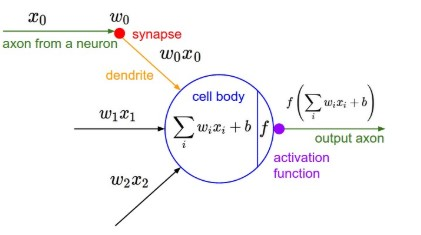
\includegraphics[width=0.70\textwidth]{CHAPTERS/Chapter-3/Images/3_1.jpg}
	\caption{Working of a single computational node}
	\label{fig:3.1}
\end{figure}

These neurons or computational nodes are organized 
into layer where there are highly interconnected to the neurons 
of following layer. The input layer of the feed forward neural 
networks feeds the information to the network and no kind of mathematical 
computation is performed. The hidden layer also known as distillation layer 
acts like a cell body and performs computation to extract salient features and 
patterns from the input data. A simple feed forward neural network with one 
hidden layer is shown in \ref{fig:3.2} \cite{chap_3_article:2}.
The output layer simply provides the results for given information. 

\begin{figure}[H]
	\centering
		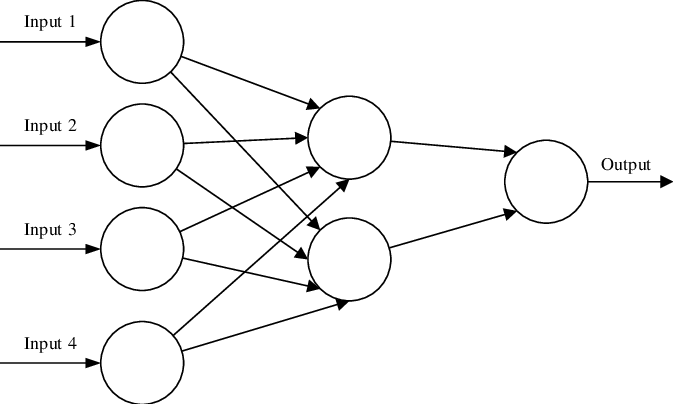
\includegraphics[width=0.70\textwidth]{CHAPTERS/Chapter-3/Images/3.2.png}
	\caption{Simple Feed Forward Neural Network with one hidden layer}
	\label{fig:3.2}
\end{figure}

The pixels of the image are arranged in a particular 
manner i.e. the appearance of the picture will be changed 
if we change the coordinate of one pixel. However, simple feed 
forward neural network loses to learn the inherent spatial 
relationships within images and fails to extract high level features 
needed for image classification. CNNs are types 
of neural networks that learn visual filters to recognize higher level 
image features and the spatial information is preserved. As a result, you 
end up learning this hierarchy of filters where filters at the early stage 
usually represents low level features like edge detection, gradient orientation 
and learning more and more complex features in the later stages.

\section{Convolutional Neural Networks Architecture}

CNNs consist of three types of layers. These layers 
include convolutional layers, pooling layers and fully connected layers. When 
these layers are stacked together, we get a CNN architecture. A general
architecture of CNNs with two convolutional layers is shown in \ref{fig:3.3} \cite{chap_3_article:2}.

\begin{figure}[H]
	\centering
		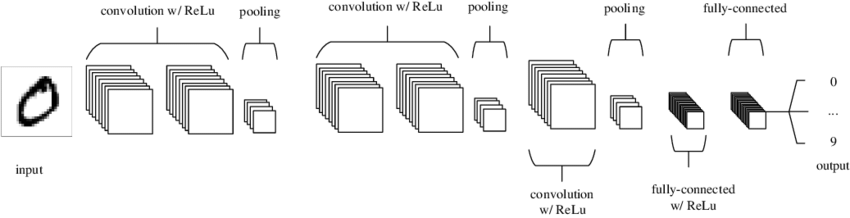
\includegraphics[width=0.80\textwidth]{CHAPTERS/Chapter-3/Images/3.3}
	\caption{Convolutional Neural Network Architecture with two convolutional layers}
	\label{fig:3.3}
\end{figure}

\subsection{Convolutional Layer}
Convolutional layers are integral part of CNNs and when these layers are stacked
 together, we start extracting more simple 
features and then aggregating these into more complex features later 
on. It consists of the set of learnable filters also known as kernels whose
height and width are smaller than the input image and always extend 
to the full depth of the input volume. We slide the filter over entire 
image to perform the mathematical operation of convolution i.e. element-wise 
multiplication of input image with the feature detector. The resultants are 
summed up and the value is assigned to the top left corner of receptive field 
as shown in figure 3.4 \cite{chap_3_article:4}.

\begin{figure}[H]
	\centering
		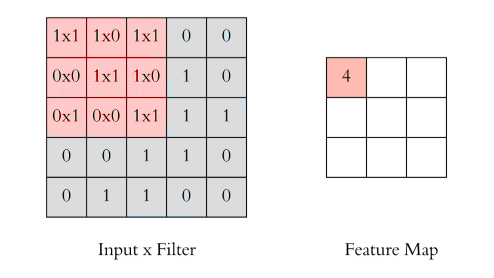
\includegraphics[width=0.70\textwidth]{CHAPTERS/Chapter-3/Images/3.4}
	\caption{3x3 filter with stride value of 1}
	\label{fig:3.4}
\end{figure}

The kernel window slides right or downward by a 
certain value in each step called the stride value and 
the process is repeated until the entire image is processed. Stride value of
1 moves the filter 1 pixel in each step. This results in a feature map with 
much smaller size than the input image and keeps on shrinking at every layer 
which is usually not desirable. Thus, dimensionality of the input image can be 
preserved by padding zero-pixel values across every side of image.

\begin{figure}[H]
	\centering
		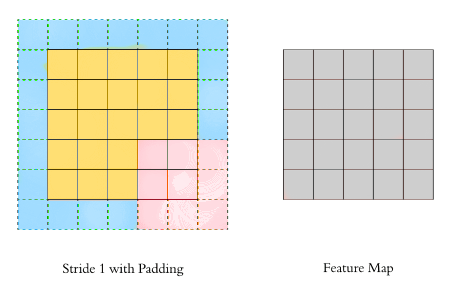
\includegraphics[width=0.70\textwidth]{CHAPTERS/Chapter-3/Images/3.5}
	\caption{Result  of 3x3 filter of Stride 1 with padding}
	\label{fig:3.5}
\end{figure}

In reality, we apply multiple filters to the same 
input image and feature maps are obtained depending upon the 
number of filters. In this case the output of convolutional layer 
is represented with a 3D matrix with dimensions of height, width 
and depth, where depth 
shows the no. of filters applied on the image. 

\begin{figure}[H]
	\centering
		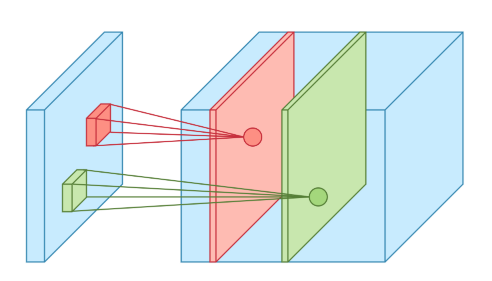
\includegraphics[width=0.70\textwidth]{CHAPTERS/Chapter-3/Images/3.6}
	\caption{Multiple filters applied on one input}
	\label{fig:3.6}
\end{figure}

\subsubsection{Activation Functions}

It is a mathematical function that is applied to every neuron 
in the network and decides whether a neuron should be activated 
or not depending on how much neuron’s input is relevant to model’s prediction. 
The main purpose of the activation function is to introduce non-linearity in the 
output. Without activation function, our network will be reduced to a simple 
regression model which would be unable to model and learn complex and complicated 
form of data. Thus, non-linear functions make neural networks capable 
of performing non-linear transformations to learn complex kinds of data such 
as 	images, videos etc. A good activation 
function should have the following properties:
\begin{itemize}
\item It should be zero centered because when back propagating gradient descent, the resulting values of gradient will either be all positive or all negative. Thus, it will affect the gradient based optimization process as we can only follow zig-zag path to reach the optimal point.
\item It shouldn’t kill the gradient flow i.e. neurons get saturated on the boundaries of activation and local gradient comes out to be zero. As a result, it nullifies the gradient flow during back propagation and dead neurons will stop updating.
\item It should be computationally efficient as activation function will be computed across millions of neurons for each input. Moreover, back propagation technique also puts constraint on the choice of activation function i.e. it should be differentiable.

\end{itemize}

\paragraph*{Sigmoid Function:}
A sigmoid function can be represented by the mathematical function:
\begin{equation}
	sig(z) = \frac{1}{1+e^{-z}}
\end{equation}
This function takes a real value as an input and squeezes 
it between 0 and -1 i.e. very large values. It is often known 
as squashing function as the large negative and positive 
values becomes 0 and 1 respectively \cite{chap_3_article:5} . However, the sigmoid function 
output is not zero-centered, and it also kills the neurons as function 
gets saturated at higher values. That’s why sigmoid function are usually 
not preferred in neural networks because of these drawbacks.

\begin{figure}[H]
	\centering
		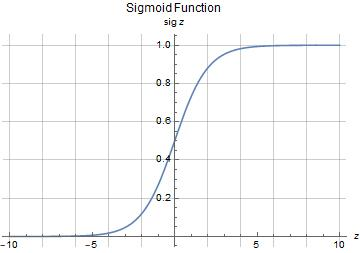
\includegraphics[width=0.70\textwidth]{CHAPTERS/Chapter-3/Images/3.7.jpg}
	\caption{Sigmoid Function}
	\label{fig:3.7}
\end{figure}
\paragraph*{Tanh Function:}
A tanh sigmoid function can be represented by the following mathematical function:
\begin{equation}
	tanh(z) = \frac{e^{z}-e^{-z}}{e^{z}+e^{-z}}
\end{equation}

It takes the real input value and squashed it between -1 and 1 i.e. very 
large negative and positive values are mapped into -1 and 1 respectively \cite{chap_3_article:5}. As 
a result, this non-linear activation function gives zero-mean data, but it 
still gets saturated at higher values as shown in \ref{fig:3.8}. However, tanh 
activations functions are preferred over sigmoid functions in neural networks.

\begin{figure}[H]
	\centering
		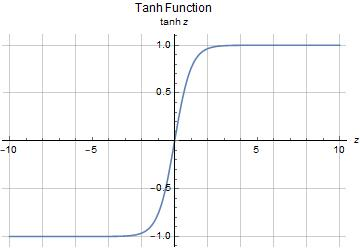
\includegraphics[width=0.70\textwidth]{CHAPTERS/Chapter-3/Images/3.8.jpg}
	\caption{Tanh function}
	\label{fig:3.8}
\end{figure}

\paragraph*{ReLU Function:}
ReLU stands for Rectified Linear unit and is represented by the following equation:

\begin{equation}
	ReLU(z) = max(0,z)
\end{equation}

It takes real values as an input and sets all the negative 
values equal to zero \cite{chap_3_article:3}. It is computationally very efficient as no 
complicated math need to be performed. And it is the most commonly used 
activation function in neural networks as it increases the convergence rate 
of gradient descent by six times as compared to sigmoid and tanh activation 
functions. However, the function doesn’t get saturated for larger values of 
inputs, but the neurons often stuck in a negative side giving zero local gradient 
and neuron will never get a chance to update in gradient descent learning process. 
This problem is also known as dying ReLU and it often occurs due to high learning 
rate or there is a large negative bias. Leaky ReLU can be used to avoid this 
situation. Leaky ReLU is very similar to original ReLU and the only difference 
is that now instead of being flat in the negative regime, we are going to give 
slight negative slope here. This solves a lot of problems we mentioned earlier
as it doesn’t saturate in the negative space and still very computationally efficient \cite{chap_3_article:3}.

% \begin{figure}
% 	\centering
% 	\begin{subfigure}{.5\textwidth}
% 	  \centering
% 	  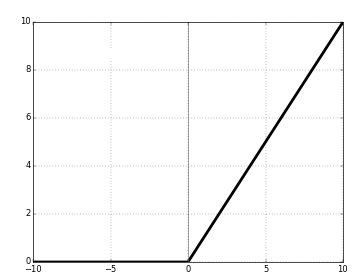
\includegraphics[width=.4\linewidth]{CHAPTERS/Chapter-3/Images/3.9a}
% 	  \caption{A subfigure}
% 	  \label{fig:3.9(a)}
% 	\end{subfigure}%
% 	\begin{subfigure}{.5\textwidth}
% 	  \centering
% 	  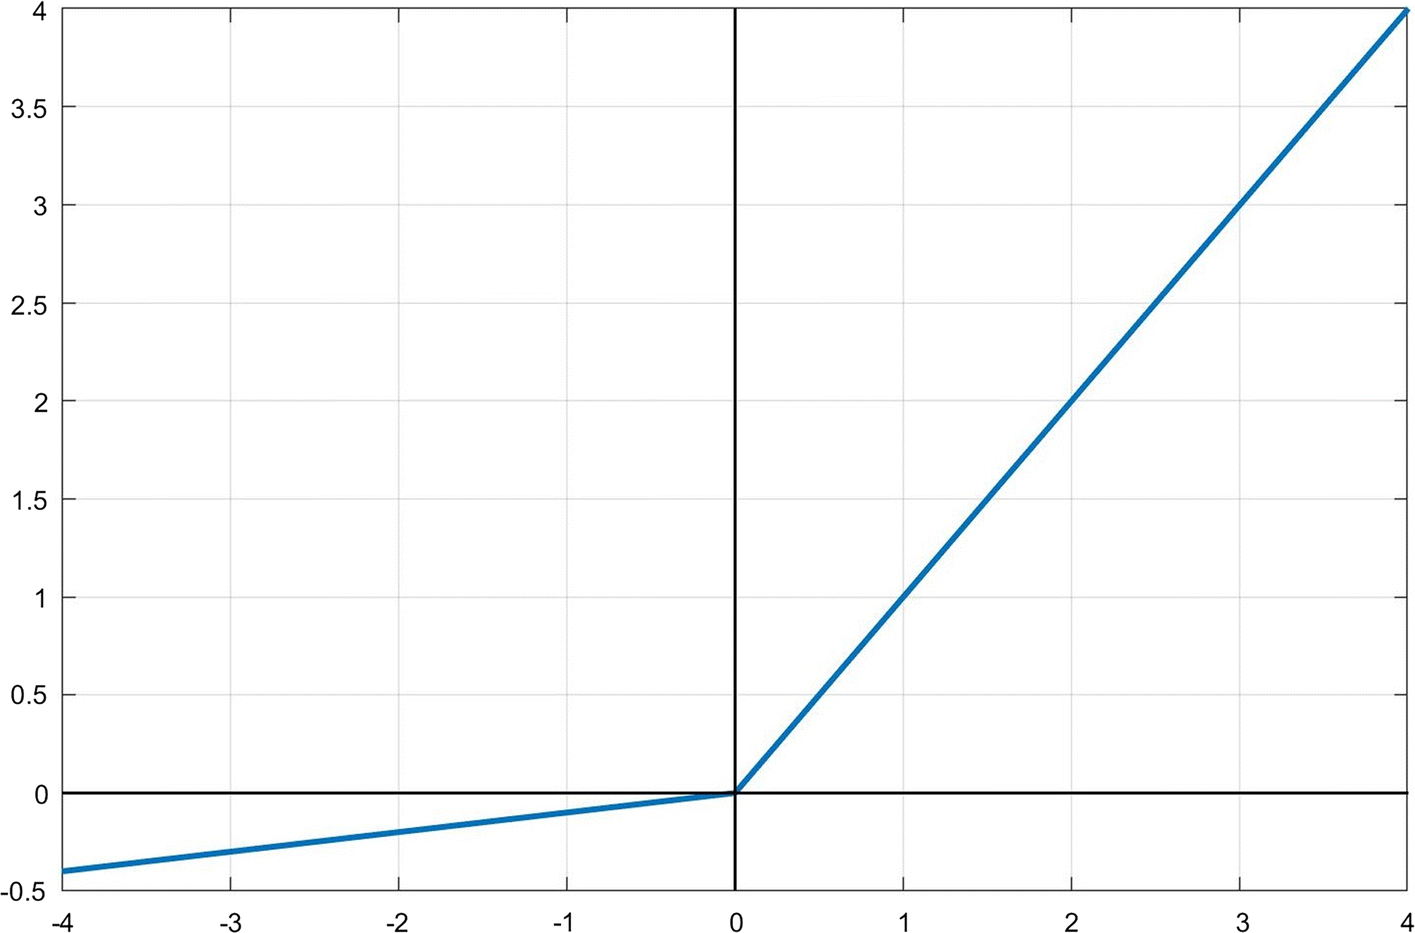
\includegraphics[width=.4\linewidth]{CHAPTERS/Chapter-3/Images/3.9b}
% 	  \caption{A subfigure}
% 	  \label{fig:3.9(b)}
% 	\end{subfigure}
% 	\caption{ReLU and Leaky ReLU Function}
% 	\label{fig:test}
% \end{figure}

\begin{figure}%
    \centering
    \subfloat[\label{fig:3.9(a)}]{{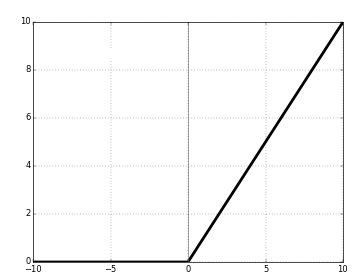
\includegraphics[height = 4.38cm, width=5cm]{CHAPTERS/Chapter-3/Images/3.9a} }}%
    \qquad
    \subfloat[\label{fig:3.9(b)}]{{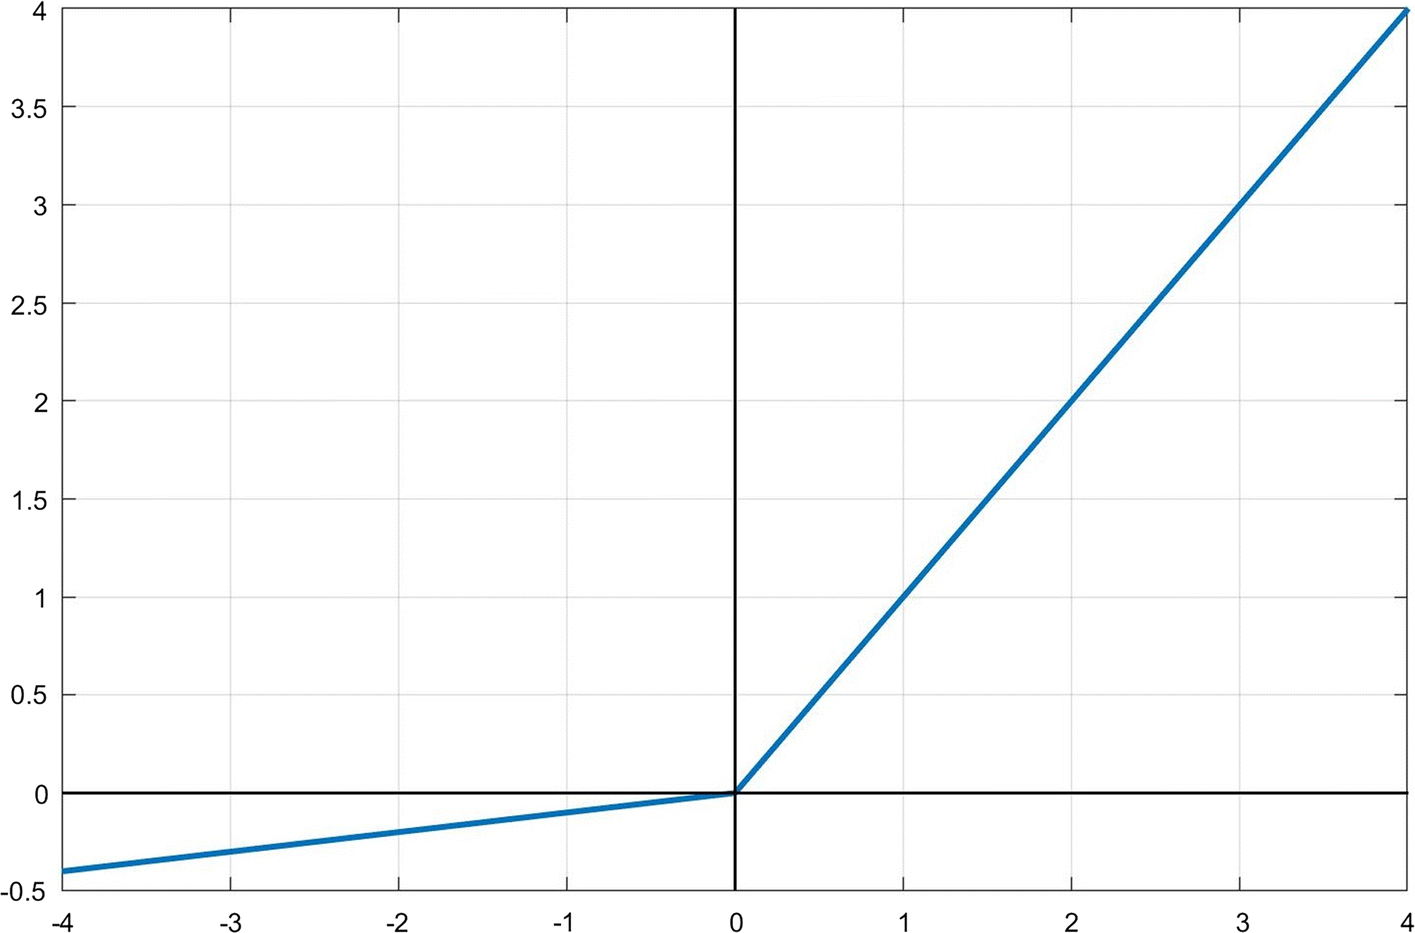
\includegraphics[height = 4cm, width=5cm]{CHAPTERS/Chapter-3/Images/3.9b} }}%
    \caption{ReLU and Leaky ReLU Function}%
    \label{fig:3.9}%
\end{figure}

\subsection{Pooling Layer}
Pooling layer follows the non-linear function introduced in convolutional layer 
in CNN. It simply down samples the feature map to 
speed up the computation as well as make some of the features it detects a bit 
more robust \cite{chap_3_article:4}. Rest of the operations will be performed on the summarized features so that the feature map is no more sensitive to the
 precise location of features in the input. Two most 
commonly used pooling techniques are described below:

\subsubsection{Average Pooling}

In average pooling, we simply place the filter window and 
find the average of pixel values covered by the filter on 
the feature map. We simply keep on sliding the filter and repeat 
the process until entire input image is processed. The average pooling 
technique with 2 x 2 filter size and 
stride value of 2 is illustrated in \ref{fig:3.10(a)}.

\subsubsection{Max Pooling}
It is a pooling technique in which the most prominent 
features in the region of feature map are retained. We simply 
take the maximum value present under filter and process the entire 
feature map to get a down-sampled output as shown in \ref{fig:3.10(b)} \cite{chap_3_article:6}.

\begin{figure}%
    \centering
    \subfloat[\label{fig:3.10(a)}]{{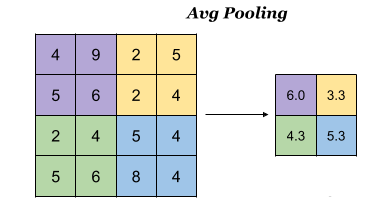
\includegraphics[height = 4cm, width=6cm]{CHAPTERS/Chapter-3/Images/3.10a} }}%
    \qquad
    \subfloat[\label{fig:3.10(b)}]{{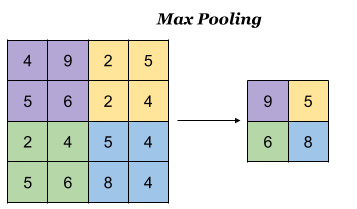
\includegraphics[height = 4cm, width=6cm]{CHAPTERS/Chapter-3/Images/3.10b} }}%
    \caption{Average and Max Pooling}%
    \label{fig:3.10}%
\end{figure}

\subsection{Flatten Layer}

The flatter layer acts as bridge between last convolutional or pooling layer 
and fully connected layer. The function of the flatten layer is to simply take
a two-dimensional feature map and stretch it into a long column vector that acts as 
an input to the fully connected layer of artificial neural network.


\begin{figure}[H]
	\centering
		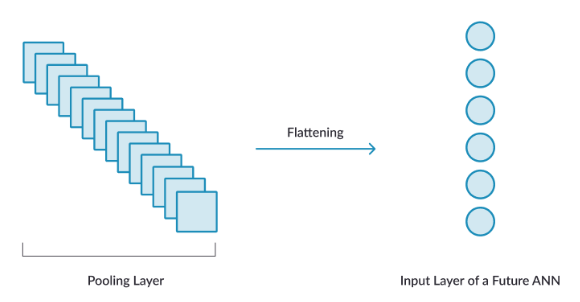
\includegraphics[width=0.60\textwidth]{CHAPTERS/Chapter-3/Images/3.11}
	\caption{Flatten layer}
	\label{fig:3.11}
\end{figure}


\subsection{Fully Connected Layer} 

Fully connected layer is considered as an important 
part of CNNs and gives the final 
probabilities for each class.  The output feature value vector obtained by the flatting layer is 
given as input to the fully connected layer. It classifies the input image into various classes using these features. The output is simply a vector 
of m $\times$ 1 dimension giving the probability of the 
classification label model is trying to predict. The probabilities of the
classes are obtained using Softman activation function which simply squashes the input values between 0 and 1 that sums to one.

Thus we conclude that CNNs are divided into two separate categories i.e. feature learning and classification. In feature learning part,
 data is passed through convolutional layer, activation functioin and pooling layer over and over again to extract several types
of features from the images. The resulting feature matrix is passed to classification
layer where it is flattened to a single vector and get probability for each class as an output of fully connected layer.
\chapter{Training \& Testing of the
Classifier}
\label{Chapter 4}
Recall from the last chapter that Convolutional Neural Networks (CNNs) are used
in the training of a model for a classifier. Classification is the process
of putting a tag on an image from a set of class labels. This chapter is about the
training of classifier for a dataset of 10000 images with 2000 images of each class.
The step by step process of training a classifier is explained in detail in this chapter. Results obtained from the testing of the classifier by varying certain parameters are recorded and attached
in the latter part of the chapter.
\section{Formation of Dataset}
In deep learning techniques for Classification of images, we have
an example of images which are input to to the system to get a
label from the given classes. This set of images is called dataset.
The dataset is divided into training and dataset by a specific ratio.


In this project we have five different classes of vehciles i.e. Bus, Car, Truck, Motorcycle
and Hiace. There are a total of 10000 images with 2000 images of each 
class. These images are downloaded from Google search results and from already available
datasets and from websites providing licensed free images like Flickr. APIs are available which
can be used along with a simple Python script to download a lot of images.
Using matplotlib in python, we can plot some of the images with the output as
shown in listing \ref{listing:4.1} and plot is attached in figure
\ref{fig:4.1}.
\begin{listing}[H]
\begin{minted}[bgcolor=bg,
    frame = lines,
    framesep = 2mm]{python}
import matplotlib.pyplot as plt
from matplotlib.image import imread  
path  = './images/'
for i in range(9):
    plt.subplot(330+1+i)
    filename = path + 'image_'+ str(i) + '.jpg'
    image = imread(filename)
    plt.imshow(image)    
    plt.show()
\end{minted}
\caption{Python script to plot some images from each class}
\label{listing:4.1}
\end{listing}

\begin{figure}[H]
    \centering
    \captionsetup{justification = centering}
    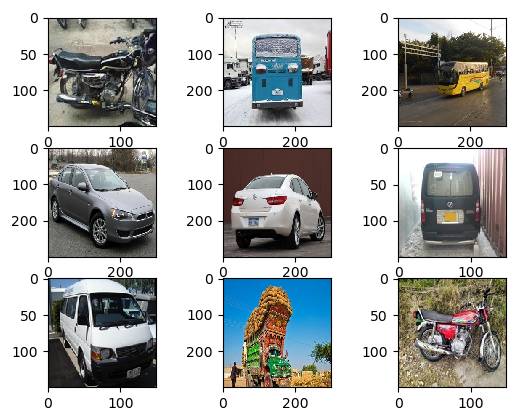
\includegraphics[scale = 0.8]{CHAPTERS/Chapter-4/Images/4.1.png}
    \caption{Plot of some images from each class} 
    \label{fig:4.1}
  \end{figure}

\subsection{Data Augmentation}
Increasing the size of dataset makes the deep learning model to learn and classify images more accurately. This problem of lack of sufficient data can be solved using technique of data augmentation which is used to increase the size of available set of images.
Data augmentation is the process of applying techniques like shifting, flipping, rotating and varying the brightness etc on images to introduce variations among them.
This technique is used within the code using Keras.
\section{Setting of Workspace for the Project}
There are a lot of images to be processed. To process images, high end GPU is
needed. Due to unavailability of an Nvidia GPU in the system, we used Google Colab.
It is an online platform having high end GPUs free provided by Google for training
up to 12 hours. Enabling a gpu in the notebook settings can accelerate the process of
training.
\section{Process of Training}
Keras is one of the leading high level API for neural networks. It contains
many modules such as layers, cost functions, activation functions, initialization
schemes and regularization schemes. This project uses Keras for training purposes.
\subsection{Conversion of Images and Labels to Numpy Arrays}
After importing all the necessary packages, we are all set to pre process our data.
Recall to chapter 2, where we studied the basics of an image. In Keras image has two
representations i.e. (width, height, color\_channels) and (color\_channels, width, height).
First approach is called as channels first approach and the latter is called as
channels last approach. We will use the channels last approach.
First step is to read the images from the folder (uploaded to Colab),
Labels are assigned to classes from 0 to 4. Keras load\_img() loads image from the folder given
target size. Target size for this project is chosen as 128 by 128. This means width and height,
both are 128. Color channels fro RGB images are 3. Images are then converted to numpy arrays using
Keras img\_to\_array() method. Labels are stored as 0, 1, 2, 3, 4 based on the class of image (as data is renamed).
A section of code for this implementation is shown in listing \ref{listing:4.2}.

\begin{listing}[H]
    \begin{minted}[bgcolor=bg,
        frame = lines,
        framesep = 2mm]{python}
folder = '/content/Input_data/'
photos = np.zeros((num_of_images,img_rows,img_cols,color_channels))
labels = np.zeros(num_of_images)
i = 0
# enumerate files in the directory
for file in os.listdir(folder):
# determine class
    if file.startswith('bus'):
        output = 0
    elif file.startswith('car'):
        output = 1
    elif file.startswith('bike'):
        output = 2
    elif file.startswith('hiace'):
        output = 3
    else:
        output = 4
    # load image
    img = load_img(folder + file, target_size=(img_rows,img_cols))
    # convert to numpy array
    img = img_to_array(img)
    # store
    images[i] = img
    labels[i] = output
    i = i+1
\end{minted}
\caption{Conversion of Images to Numpy arrays}
\label{listing:4.2}
\end{listing}
The images array has a pattern (num\_of\_images, rows, cols, color\_channels). It
means that it has a shape (10000, 128, 128, 3). This is a 4D tensor. There are 10000
images with each image having 128, $128\times 3$ matrices i.e. each $128\times 3$ matrix has
128 rows with each row containing 3 columns with information of 3 colors.
The labels array is a 1D tensor with 10000 \% labels.
\subsection{Train-Test Division}
We have to divide the data into two parts, train and test. The training data
is used to for training purposes and when the model is trained then it is
used to test the model using the test images and test labels. We used a ratio of 75\% and
25\% for train and test respectively. The package used for this purpose is the
Scikit-learn train\_test\_split. Listing \ref{listing:4.3} shows splitting of
data into train and test.

\begin{listing}[H]
    \begin{minted}[bgcolor=bg,
        frame = lines,
        framesep = 2mm]{python}
train_images, test_images, train_labels, test_labels = 
train_test_split(images, labels, test_size = 0.25, random_state = 42)
\end{minted}
\caption{Train-test split}
\label{listing:4.3}
\end{listing}
There is another technique for splitting of data. We make two directories
train and test and randomly divide the images into these directories and then
convert them into numpy array. Here we have first converted the images
into arrays, split them into train and test and then we can save them back into
directories by converting them into images from array using PIL from\_array
function.

\subsection{Mean Correction}
After converting to float 32 and normalizing by 255, we have to subtract mean pixel.
Listing \ref{listing:4.4} illustrates the mean correction.

\begin{listing}[H]
    \begin{minted}[bgcolor=bg,
        frame = lines,
        framesep = 2mm]{python}
if subtract_pixel_mean:
x_train_mean = np.mean(train_images, axis=0)
train_images -= x_train_mean
test_images -= x_train_mean
train_labels = to_categorical(train_labels,num_classes)
test_labels = to_categorical(test_labels,num_classes)
    \end{minted}
    \caption{Mean correction}
\label{listing:4.4}
\end{listing}
\noindent The last two lines are categorical labeling for using labels fit for Keras.
\subsection{Defining the Model}
Recall from chapter \ref{Chapter 3}, a CNN model consists of various layers including
conv2D, Activation, MaxPoooling2D, Flatten and Dense layer. Listing \ref{listing:4.5}
defines the training Model.

\begin{listing}[H]
    \begin{minted}[bgcolor=bg,
        frame = lines,
        framesep = 2mm]{python}
#Model
model = Sequential()
model.add(Conv2D(32, (3, 3), padding='same',
                         input_shape=train_images.shape[1:]))
model.add(Activation('relu'))
model.add(Conv2D(32, (3, 3)))
model.add(Activation('relu'))
model.add(MaxPooling2D(pool_size=(2, 2)))
model.add(Dropout(0.25))   
model.add(Conv2D(64, (3, 3), padding='same'))
model.add(Activation('relu'))
model.add(MaxPooling2D(pool_size=(2, 2)))
model.add(Dropout(0.25))      
model.add(Flatten())     
model.add(Dense(64))
model.add(Activation('relu'))
model.add(Dropout(0.5))      
model.add(Dense(num_classes))
model.add(Activation('softmax'))      
model.compile(loss='categorical_crossentropy',
                      optimizer='adam',
                      metrics=['accuracy'])
    \end{minted}
    \caption{Defining the Model}
\label{listing:4.5}
\end{listing}
Last three lines defines the compilation process of the Model. 
For more than two classes, loss is categorical\_crossentropy. For two
classes it is binary\_crossentropy. There are many optimizers in Keras i.e.
SGD, Adam, RMSprop, Adamax etc. Here we have used Adam. Metrics calculates how
often prediction equals labels.
\subsection{Fitting the Model}
Here the process of training starts. We have two functions used in Keras. One
is model.fit and other is model.fit\_generator. As we discussed in section 4.1.1
about data augmentation. Here we have implemented data augmentation using a true false
logic. We have also defined a validation set. Validation data tells us about the
behavior of the model to an unseen data.

The number of times a model goes through the data is termed as `epochs'.
We have to determine the specific number of epochs for which the training process has to
run. If we run the process above that number, the training accuracy will
increase. But when we test that model with the test data, the accuracy of the model
will be lower than the training accuracy. This process is called `\textit{overfitting}'.
We have to avoid the overfitting. We use validation data which shows us the validation accuracy
and loss after each epoch. Listing \ref{listing:4.6} shows the code for training process.
\begin{listing}[H]
    \begin{minted}[bgcolor=bg,
        frame = lines,
        framesep = 2mm]{python}
if subtract_pixel_mean:
x_train_mean = np.mean(train_images, axis=0)
train_images -= x_train_mean
test_images -= x_train_mean
train_labels = to_categorical(train_labels,num_classes)
test_labels = to_categorical(test_labels,num_classes)
    \end{minted}
    \caption{Mean correction}
\label{listing:4.4}
\end{listing}
\noindent The last two lines are categorical labeling for using labels fit for Keras.
\subsection{Defining the Model}
Recall from chapter \ref{Chapter 3}, a CNN model consists of various layers including
conv2D, Activation, MaxPoooling2D, Flatten and Dense layer. Listing \ref{listing:4.7}
defines the training Model.

\begin{listing}[H]
    \begin{minted}[bgcolor=bg,
        frame = lines,
        framesep = 2mm]{python}
if not data_augmentation:
    print('Not using data augmentation.')
    history = model.fit(train_images, train_labels, validation_data=(test_images,
    test_labels), batch_size = batch_size, epochs = n_epochs)
else:
    datagen = ImageDataGenerator(
        featurewise_center=False,  # set input mean to 0 over the dataset
        samplewise_center=False,  # set each sample mean to 0
        featurewise_std_normalization=False,  # divide inputs by std of the dataset
        samplewise_std_normalization=False,  # divide each input by its std
        zca_whitening=False,  # apply ZCA whitening
        zca_epsilon=1e-06,  # epsilon for ZCA whitening
        rotation_range=0,  # randomly rotate images in the range (degrees, 0 to 180)
        width_shift_range=0.1,
        height_shift_range=0.1,
        shear_range=0.,  # set range for random shear
        zoom_range=0.,  # set range for random zoom
        channel_shift_range=0.,  # set range for random channel shifts
        fill_mode='nearest',
        cval=0.,  # value used for fill_mode = "constant"
        horizontal_flip=True,  # randomly flip images
        vertical_flip=False,  # randomly flip images
        rescale=None,
        preprocessing_function=None,
        # image data format, either "channels_first" or "channels_last"
        data_format=None,
        validation_split=0.0)
        datagen.fit(train_images)
        history = model.fit_generator(datagen.flow(train_images, train_labels,
        batch_size = batch_size),validation_data=(test_images, test_labels),
        epochs = n_epochs)  
    \end{minted}
    \caption{Training the Model}
\label{listing:4.7}
\end{listing}
\subsection{Plotting the Accuracy and Loss}
A specific model has a specific accuracy upto which it can detect an unknown data.
Increasing epochs will not increase the accuracy, it basically overfits
the model. For a certain model, we have to find a specific number
of epochs. For this we plot the accuracy and loss of training and
validation data.

Listing \ref{listing:4.8} shows the script for plotting the accuracy and
loss of training and validation data.

\begin{listing}[H]
    \begin{minted}[bgcolor=bg,
        frame = lines,
        framesep = 2mm]{python}
plt.grid()
plt.plot(history.history['acc'])
plt.plot(history.history['val_acc'])
plt.title('model accuracy')
plt.ylabel('accuracy')
plt.xlabel('epoch')
plt.legend(['train', 'validation'], loc='upper left')
plt.show()
# summarize history for loss
plt.grid()
plt.plot(history.history['loss'])
plt.plot(history.history['val_loss'])
plt.title('model loss')
plt.ylabel('loss')
plt.xlabel('epoch')
plt.legend(['train', 'val'], loc='upper left')
plt.show()
\end{minted}
\caption{Training, validation accuracy \& loss vs. epochs}
\label{listing:4.8}
\end{listing}

\subsection{Saving Model \& Weights}
After successful training of model, we have to resuse it. We can directly test it for one time
when the Colab is not recycled. So the better approach is to save the model
and then evalaute it on test data. Model is stored as .h5 file in the root directory.
Listing \ref{listing:4.9} shows the script for saving the weights.

\begin{listing}[H]
    \begin{minted}[bgcolor=bg,
        frame = lines,
        framesep = 2mm]{python}
# Save model and weights
if not os.path.isdir(save_dir):
    os.makedirs(save_dir)
model_path = os.path.join(save_dir, model_name)
model.save(model_path)
print('Saved trained model at %s ' % model_path)
\end{minted}
\caption{Saving the Model}
\label{listing:4.9}
\end{listing}
\section{Evaluation of Model}
Loading the Model saved in the root directory and test it using evalaute function
tells us the accuracy of Model on the test data. Listing \ref{listing:4.10} shows the script for
evalaution.
\begin{listing}[H]
    \begin{minted}[bgcolor=bg,
        frame = lines,
        framesep = 2mm]{python}
#Load Model
loaded_model = load_model("saved_models/model.h5")
#Evaluate Model
test_loss, test_acc = loaded_model.evaluate(test_images, test_labels)
print('Accuarcy of the model:', test_acc)
\end{minted}
\caption{Evaluating the Model}
\label{listing:4.10}
\end{listing}

\addappheadtotoc
%\appendixpage
% \begin{appendices}
% \chapter{Linear Matrix Inequalities} 
     \section{Simple Approach}
     
     \section{Generalized Eigenvalue Problem}

% \chapter{Array Processing} 
     \section{Types of Arrays}
     
     \section{Constraints in Array Processing}

% \end{appendices}
% include your .bib file

\renewcommand{\bibname}{References}
\cleardoublepage
\phantomsection
\addcontentsline{toc}{chapter}{References}

\bibliography{thesis}
\bibliographystyle{IEEEtr}
%\cleardoublepage
\phantomsection
\addcontentsline{toc}{chapter}{About the Author}

\begin{center}
\huge  About the Author
\vspace{0.5in}
\begin{figure}[h]
	\centering
		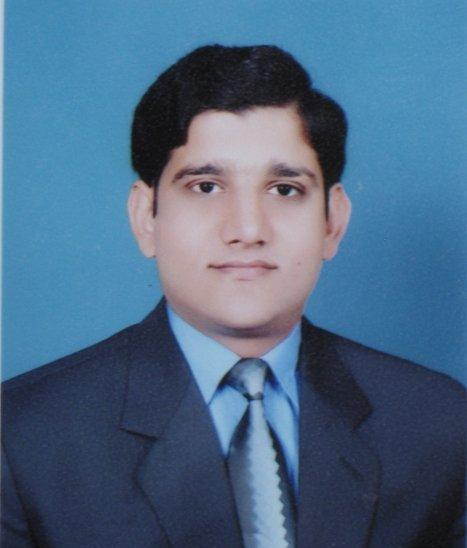
\includegraphics[width=0.50\textwidth]{back/about_the_author/about_the_author.jpg}
	\label{fig:about_the_author}
\end{figure}
\vspace{0.4in}
\normalfont
\end{center}
%% write text here

The author is member of Pasking Group. 
\end{document}
